%!TEX root = ../report.tex
Section\section{Feature extraction} % (fold)
\label{sec:feature_extraction}
The goal of this chapter is to explain how the ball used as the tracking object was detected in both images. With these positions the stereopsis can be computed as explained in \ref{sec:stereopsis} and hence the 3D position of the ball in the world can be obtained.
The tracking of the object was a function implemented inside the node "balltracker" explained in section \ref{sec:structure}.

\subsection{Methods}
For detecting the balls in both images the first approach was to user the opencv function "blur" to smooth the image in order to avoid having lots of very small contours with a kernel of 9x9 pixels. After this action the image was converted from RGB colorspace to HSV one. The reason for this is that generally is much simpler and precise to do color segmentation in the HSV colorspace rather than in RGB. This segmentation was performed using the opencv function "inrange" with minimum and maximum limits of 25 to 100 for hue, 70 to 255 for saturation and 100 to 255 for value. This process produced a binary image with some small artifacts spread in the image and the object to detect with some holes inside as it can be seen in figure \ref{fig:binary_image}.
 
\begin{figure}[h]
    \centering
    %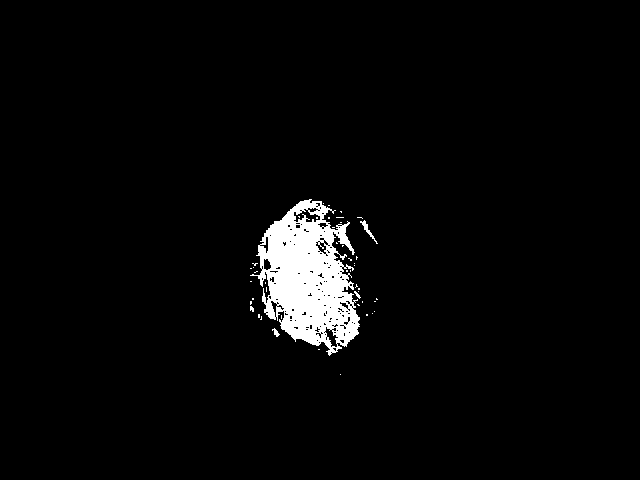
\includegraphics[width=0.8\textwidth]{images/binary.png}
    \caption{Binary image obtained after applying color threshold}
    \label{fig:binary_image}
\end{figure}

For removing those artifacts an opening morphological operation was performed with a kernel size of 9x9 pixels. Once the undesired objects were erased by the previous operation, a closing morphological operation was applied in order to remove the holes inside the object to be detected with the same kernel size. The result of these operations can be seen in figure \ref{fig:filtered_image}.

\begin{figure}[h]
    \centering
    %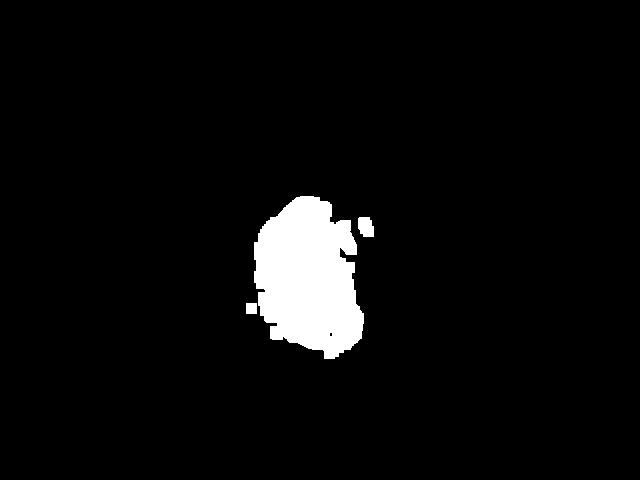
\includegraphics[width=0.8\textwidth]{images/filtered.png}
    \caption{Binary image obtained after applying the morphological operations}
    \label{fig:filtered_image}
\end{figure}

Once that the image is clean enough the opencv function "findcontours" is used, and for every contour that it detects the arc length and area are computed. Then, a radius threshold is applied to these contours. The value selected for the threshold is 30 pixels, and it was obtained by trial and error. Given the area and perimeter of the contours the threshold is applied following the equations \ref{eq:circ_area} and \ref{eq:circ_perimeter}.

\begin{equation}
area_{contour}>2*\pi*radius_{threshold}^{2}
\label{eq:circ_area}
\end{equation}

\begin{equation}
perimeter_{contour}>2*\pi*radius_{threshold}
\label{eq:circ_perimeter}
\end{equation}

Following, the circularity of the contours that have a radius bigger than the threshold is computed following equation \ref{eq:circularity}. Then, the moments of the ones that have a circularity bigger than 0,2 are computed and hence, their centroids are extracted and sent to the stereopsis function of the node. Again, the value of 0,2 for the circularity was extracted by trial and error. The value is rather low because the output of the previous filtering phases doesn't keep a circular shape properly.

\begin{equation}
circularity=\frac{4*\pi*area_{contour}}{perimeter_{contour}^{2}}
\label{eq:circularity}
\end{equation}

\subsection{Results}
Several variations of the algorithm stated above were tested before ending up with that one. However, the original ball given as a marker to be tracked was completely white. Therefore, as the laboratory where the workcells are situated has high ceilings and the only windows are close to them, the sun was hitting with a high angle. This illumination configuration produced very bright spots on the top of the ball (easily seen by the cameras) while the rest of the ball stayed with less brightness. In addition, the walls surrounding the workcell are mainly white and, at certain moments of the day very bright. Consequently, tracking the white ball was a very difficult task. To fix this issue, the ball was covered with a piece of green paper that made the colour detection easier. Nevertheless, the high inclination of the sun still produced a spot of higher brightness in the top of the ball that wasn't detected by the algorithm. For fixing this, the closing morphology operation was performed as explained in the section above, which provided a much circular shape to the ball in the image than the one obtained by simply thresholding.
All in all, the final detection of the ball was stable enough to provide consistent data for the stereopsis and the trajectory prediction.

% section feature_extraction (end)~\ref{sec:}